\documentclass[a4paper,10pt]{article}

\usepackage[bottom=0.5cm]{geometry}

%A Few Useful Packages
\usepackage{marvosym}
\usepackage{fontspec} 					%for loading fonts
\usepackage{xunicode,xltxtra,url,parskip} 	%other packages for formatting
\RequirePackage{color,graphicx}
\usepackage[usenames,dvipsnames]{xcolor}
\usepackage[big]{layaureo} 				%better formatting of the A4 page
% an alternative to Layaureo can be ** \usepackage{fullpage} **
\usepackage{supertabular} 				%for Grades
\usepackage{titlesec}					%custom \section

%Setup hyperref package, and colours for links
\usepackage{hyperref}
\definecolor{linkcolour}{rgb}{0,0.2,0.6}
\hypersetup{colorlinks,breaklinks,urlcolor=linkcolour, linkcolor=linkcolour}
\urlstyle{same}

%Defined width table colums that work like l, c and r.
\usepackage{array}
\newcolumntype{L}[1]{>{\raggedright\let\newline\\\arraybackslash\hspace{0pt}}m{#1}}
\newcolumntype{C}[1]{>{\centering\let\newline\\\arraybackslash\hspace{0pt}}m{#1}}
\newcolumntype{R}[1]{>{\raggedleft\let\newline\\\arraybackslash\hspace{0pt}}m{#1}}
\newcolumntype{D}{>{\raggedleft\let\newline\\\arraybackslash\hspace{0pt}}m{1.51cm}}



%FONTS
\defaultfontfeatures{Mapping=tex-text}
%\setmainfont[SmallCapsFont = Fontin SmallCaps]{Fontin}
%%% modified for Karol Kozioł for ShareLaTeX use
\setmainfont[
SmallCapsFont = Fontin-SmallCaps.otf,
BoldFont = Fontin-Bold.otf,
ItalicFont = Fontin-Italic.otf
]
{Fontin.otf}

\newfontfamily\namefont{Times New Roman}%Quattrocento-Regular.ttf}

\usepackage{anyfontsize}	%set any font size (duh)

%%%

%CV Sections inspired by: 
%http://stefano.italians.nl/archives/26
\titleformat{\section}{\Large\scshape\raggedright}{}{0em}{}[\titlerule]
\titlespacing{\section}{0pt}{3pt}{3pt}

%Tweak a bit the top margin
\addtolength{\voffset}{-0.4cm}



%Italian hyphenation for the word: ''corporations''
\hyphenation{im-pre-se}

%-------------WATERMARK TEST [**not part of a CV**]---------------
%\usepackage[absolute]{textpos}

%\setlength{\TPHorizModule}{30mm}
%\setlength{\TPVertModule}{\TPHorizModule}
%\textblockorigin{2mm}{0.65\paperheight}
%\setlength{\parindent}{0pt}

%--------------------BEGIN DOCUMENT----------------------
\begin{document}

%WATERMARK TEST [**not part of a CV**]---------------
%\font\wm=''Baskerville:color=787878'' at 8pt
%\font\wmweb=''Baskerville:color=FF1493'' at 8pt
%{\wm 
%	\begin{textblock}{1}(0,0)
%		\rotatebox{-90}{\parbox{500mm}{
%			Typeset by Alessandro Plasmati with \XeTeX\  \today\ for 
%			{\wmweb \href{http://www.aleplasmati.comuv.com}{aleplasmati.comuv.com}}
%		}
%	}
%	\end{textblock}
%}

\pagestyle{empty} % non-numbered pages

\font\fb=''[cmr10]'' %for use with \LaTeX command

%--------------------TITLE-------------
{  \Huge \namefont {\fontsize{35}{0}\namefont C}LAES {\fontsize{35}{0}\namefont A}NDERSSON} \bigskip\par

%--------------------SECTIONS-----------------------------------
%Section: Personal Data
\section{Personal Data}

\begin{picture}(0,0) 
\put(272,-96){\hbox{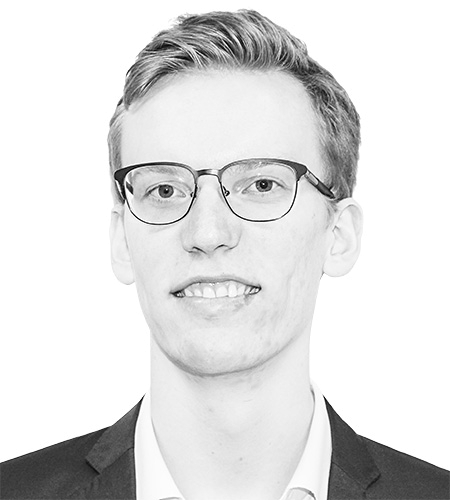
\includegraphics[scale=0.4]{profile}}}
\end{picture}

\begin{tabular}{Dl}
    \textsc{Address:}	&	 Vänortsvägen 5, Luleå, Sweden \\
    \textsc{Phone:}		&	 +46 73 763 87 77\\
    \textsc{email:}		&	 \href{mailto:Claes.Gustaf.Andersson@gmail.com}{Claes.Gustaf.Andersson@gmail.com}\\
    \textsc{Linkedin:}	&	 \url{se.linkedin.com/in/ClaesGustaf} \\
    \textsc{GitHub:}		&	 \href{https://github.com/Fizzr}{GitHub.com/Fizzr}
\end{tabular}

\section{Goal}
{\small The main goal in my career is to learn. I want to be challenged in a way that forces me to learn new things and think in new ways. I want to become the best in my field at what I do, and I want to be a part of creating flawless and perfect solutions!}

%Section: Education
\section{Education}
\begin{tabular}{D L {\textwidth - 2.7cm}}
\textsc{Jun 2018}	&	\textbf{Computer Engineering Master's Degree}\\
\textsc{Aug 2012}	&	 \emph{Information and Communication Technology}. Luleå Tekniska Universitet.\\
			&	{\small Focus on Algorithms, Design paradigms, high levels of abstraction, Networking, and Internet services and development.}
\end{tabular}


%Section: Work Experience
\section{Work Experience}
\begin{tabular}{D L {\textwidth - 2.7cm}}
 \emph{Current} 	& 	\textbf{Brand Ambassador}	\\
 \textsc{Mar 2015}	&	Academic Work			\\
 			&	{\small Tasked with maintaining and promoting the brand ``Academic Work'' and slogan ``Home of the Young Professional'' on campus. A job requiring effortless socializing with both strangers and colleagues, independent effort but also to be able to work together in tight groups, and to always appear professionally.}	\\
			&						\\
\emph{Current}	&	\textbf{Co-founder}		\\
\textsc{Sep 2013}	&	DC Technological Innovations HB	\\
 			&	{\small A company created in attempts to bring the crypto-currency Bitcoin to our university and make it the dominant payment method within campus. Now mostly idle.  }					\\
 			&						\\
\textsc{Aug 2016}	&	\textbf{Junior Developer}		\\
\textsc{Jun 2016}	&	isMobile				\\
			&	{\small Worked as a consultant through Academic Work. Worked with developing a demo suite for their Android Application Module. Worked primarily in XSLT, HTML, JavaScript and Java}	\\
			

\end{tabular}


%Section: Languages
\section{Languages}
\begin{tabular}{Dl}
 \textsc{Swedish:}&Mother tongue\\
\textsc{English:}&Fluent\\
\end{tabular}

\section{Computer Skills}
\begin{tabular}{rl}
\textsc{ Traditional Languages:}		&	C/++/\#, Java, Python\\
\textsc{Web Development:}		&	 HTML, JavaScript,  PHP, MySQL, CSS\\
\textsc{Other:}				& 	LaTeX, XML, XSLT, JSON, Git\\
\textsc{Environments:}			&	Android, Unity, 3ds Max, Office\\
\textsc{Touched on: }			&	Go!, Prolog, Haskell, Assembly, VHDL
\end{tabular}
\\[0.3cm]

\centering\textsc{ References left on request}

\end{document}
